\documentclass[12pt]{beamer}
\usepackage[english, russian]{babel}
\usepackage[utf8x]{inputenc}
\usepackage{itmobeamer}
\usepackage{makecell}
\usepackage{tabularx}
\usepackage{multicol}
\usepackage{caption}
\usepackage{listings}
\usepackage{subcaption}
\usepackage[export]{adjustbox}

\lstset{emph={
    tc, qdisc, class, dev, parent, classid, filter, protocol, flowid, cbwfq, default, bandwidth,
    },emphstyle={\bfseries}%
}%

\title[Реализация CBWFQ в ядре Linux]{Реализация дисциплины обслуживания CBWFQ для ядра Linux\\}
\author[]{{\small Автор: Куклина Мария Дмитриевна\\ Научный руководитель: Шинкарук Дмитрий Николаевич\\}}
\institute[]{Университет ИТМО}
\date[]{Санкт-Петербург, 2018}

\setbeamertemplate{caption}[numbered]

\begin{document}

\setcounter{figure}{0}

\newcommand{\mc}[0]{\makecell}
\newcommand\setrow[1]{\gdef\rowmac{#1}#1\ignorespaces}
\newcommand\clearrow{\global\let\rowmac\relax}
\clearrow
%\itmologoslide

\begin{darkbars}
    \begin{frame}[noheader,nologo,noframenumbering]
        \titlepage
    \end{frame}
\end{darkbars}

\begin{frame}{Цели и задачи}
    \textbf{Цель} -- реализация дисциплины обслуживания Class-Based Weighted Fair Queueing
    (CBWFQ) в ядре Linux. \newline

    \textbf{Задачи}
    {\small
        \begin{itemize}

    \item Проанализировать и сравнить дисциплины обслуживания PQ, CBQ, HTB, HFSC, FWFQ, CBWFQ.
    \item Восстановить алгоритмы Class-Based WFQ.
    \item Настроить среду для реализации и тестирования.
    \item Реализовать модуль ядра CBWFQ в ядре Linux.
    \item Реализовать интерфейс утилиты tc для управления модулем.
    \item Провести тестирование.
        \end{itemize}
    }
\end{frame}

\begin{frame}{Сравнительная таблица ДО}
{\scriptsize
        \begin{tabular}{|>{\rowmac}c|>{\rowmac}c|>{\rowmac}c|>{\rowmac}c|>{\rowmac}c|>{\rowmac}c|>{\rowmac}c<{\clearrow}|}
            \hline
            \setrow{\bfseries}     Свойство        & PQ   & CBQ   & HTB   & HFSC  & FWFQ  & CBWFQ \\ \hline
            {\bf \mc{Метод\\ планирования        }}& RR   & WRR   & RR    & RT/LS & WFQ   & WFQ   \\ \hline
            {\bf Отбрасывание                     }& TD   & TD    & TD    & TD    & ED/AD & TD/WRED \\ \hline
            {\bf \mc{Честность}}& -    & -     & -     & -     &  +    &  +    \\ \hline
            {\bf \mc{Разделение\\ канала         }}& -    &  +    &  +    &  +    &  -    &  -    \\ \hline
			{\bf \mc{Решение проблемы\\ голодания}}& -    &  +    & +     & +     & +     & +    \\ \hline
            {\bf \mc{Сложность \\ реализации     }}& Низк & Выс   &Сред   & Выс   & Сред  & Сред \\ \hline
            {\bf \mc{Сложность \\ конфигурации   }}& Низк & Выс   &Сред   & Выс   & Низк  & Низк \\ \hline
            {\bf \mc{Конфигурация\\ классов      }}& -    & +     & +     & +     & -     & + \\ \hline
            {\bf \mc{Реализация\\ в Linux        }}& +    & +     & +     & +     & -     & -  \\ \hline
        \end{tabular}
}
{\scriptsize
	Обозначения:
	 (W)RR -- (Weighted) Round Robin, RT/LS -- Real Time/Link Sharing.
	 TD -- Tail Drop, ED/AD -- Early Dropping/Aggressive Dropping.
}
\end{frame}

\begin{frame}{Качество обслуживания в ядре Linux}
	\begin{figure}
		\center
    	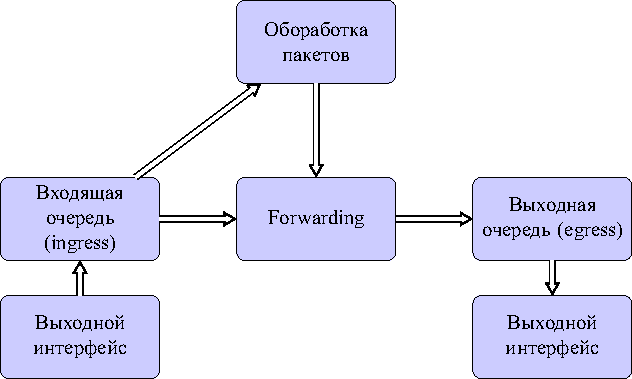
\includegraphics[scale=0.8]{../text/pdfimages/qdisc.pdf}
		\caption*{Схема движения пакетов в ядре Linux.}
	\end{figure}
\end{frame}

\begin{frame}{WFQ на основе вычисления порядкового номера пакета}
	\begin{figure}
		\center
    	\includegraphics[scale=0.7]{../text/pdfimages/wfq_seq.pdf}
		\caption*{}
	\end{figure}
\end{frame}

\begin{frame}{Class-Based Weighted Fair Queueing}
	\begin{figure}
		\center
    	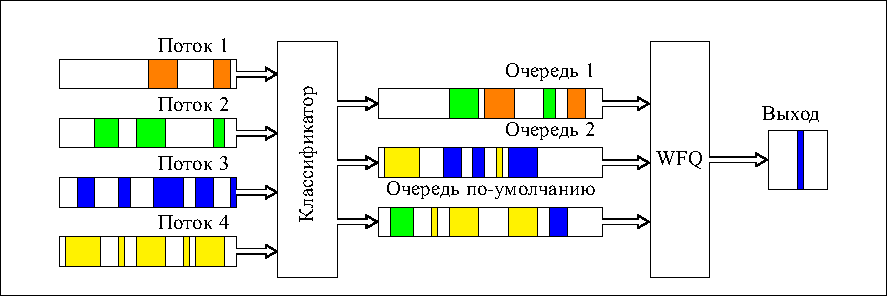
\includegraphics[scale=0.8]{../text/pdfimages/cbwfq.pdf}
		\caption*{Схема движения пакетов в планировщике CBWFQ}
	\end{figure}

	\begin{center}
{\footnotesize
	\begin{itemize}
		\item Возможность конфигурации пользовательских классов.
		\item Выделение минимальной пропускной способности классу.
	\end{itemize}
}
	\end{center}
\end{frame}


\begin{frame}{Блок-схемы алгоритмов CBWFQ}
	\begin{figure}[t]
		\begin{subfigure}[b]{0.4\textwidth}
            \center
            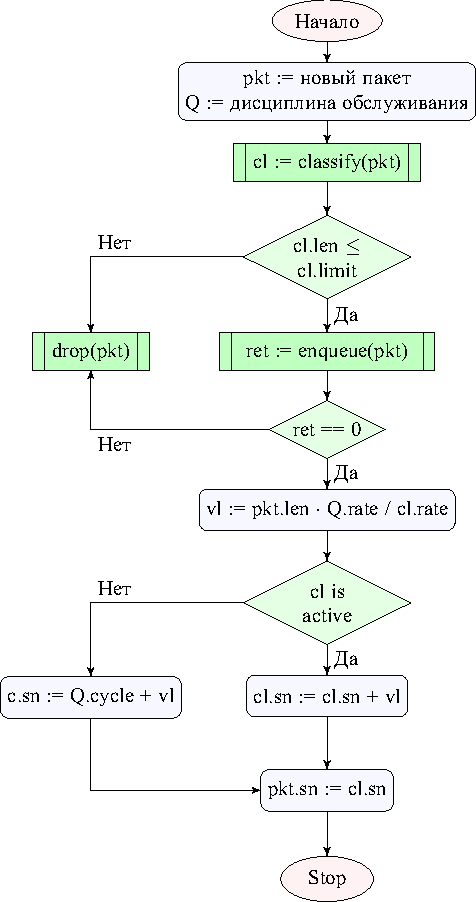
\includegraphics[scale=0.45,frame]{../text/pdfimages/enq_algo.pdf}%
    		\caption*{Алгоритм enqueue}
		\end{subfigure}
~~~~~~~~
		\begin{subfigure}[b]{0.4\textwidth}
            \center%
            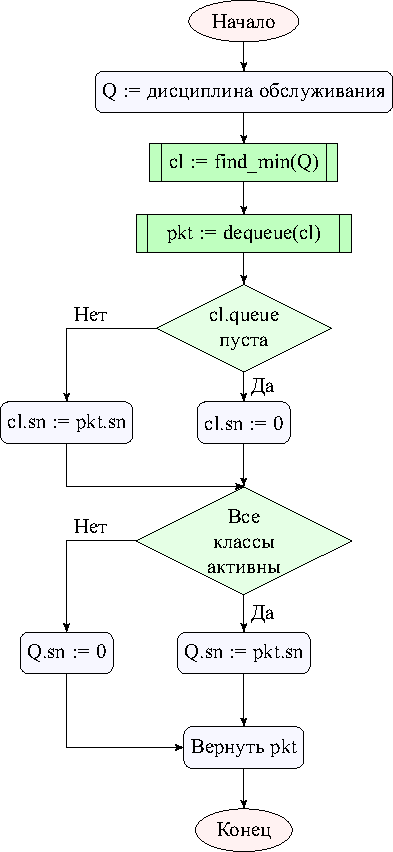
\includegraphics[scale=0.5,frame]{../text/pdfimages/deq_algo.pdf}%
    		\caption*{Алгоритм dequeue}
		\end{subfigure}
	\end{figure}	
\end{frame}

\begin{frame}[fragile]{Настройка тестовой среды}
	\begin{figure}[t]
		\center
    	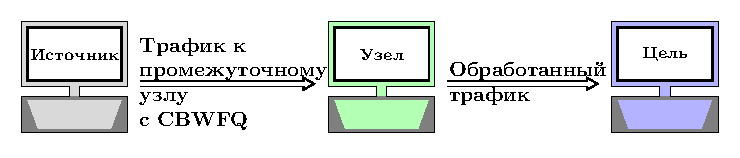
\includegraphics[scale=0.8]{../text/pdfimages/test_scheme.pdf}
	\end{figure}
{\footnotesize
	\begin{lstlisting}[frame=single]
tc qdisc add dev $IFACE root handle 1: cbwfq bandwidth\
        100Mbps default rate 5Mbps
tc class add dev $IFACE parent 1: classid 1:2 cbwfq   \
        rate 70Mbps
tc class add dev $IFACE parent 1: classid 1:3 cbwfq   \
        rate 25Mbps
tc filter add dev ens4 parent 1:1 protocol ip u32 match \
        ip dport $TESTPORT1 0xffff flowid 1:2
tc filter add dev ens4 parent 1:0 protocol ip u32 match \
        ip dport $TESTPORT2 0xffff flowid 1:3
    \end{lstlisting}
}
%
\end{frame}

\begin{frame}[fragile]{Структура эксперимента №1}

{\footnotesize
	\begin{lstlisting}[frame=single,emph={iperf3},emphstyle={\bfseries}]
iperf3 -c $SERVERIP1 -p $TESRPORT1 -b 500M -u -t 90
iperf3 -c $SERVERIP2 -p $TESRPORT2 -b 500M -u -t 90
    \end{lstlisting}
}%
	\begin{figure}
		\center
    	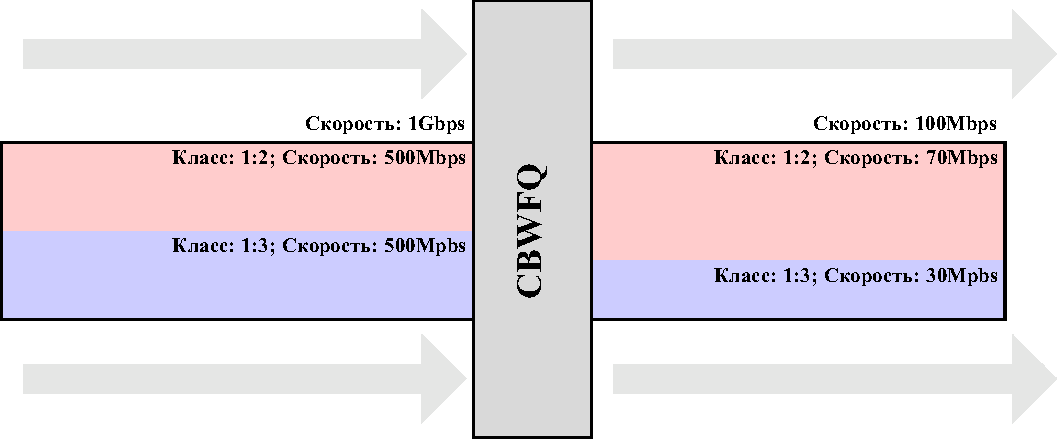
\includegraphics[scale=0.65]{../text/pdfimages/exp_scheme.pdf}
	\end{figure}
\end{frame}

\begin{frame}{График распределения доли ПС по классам}
	\begin{figure}[t]
		\center
    	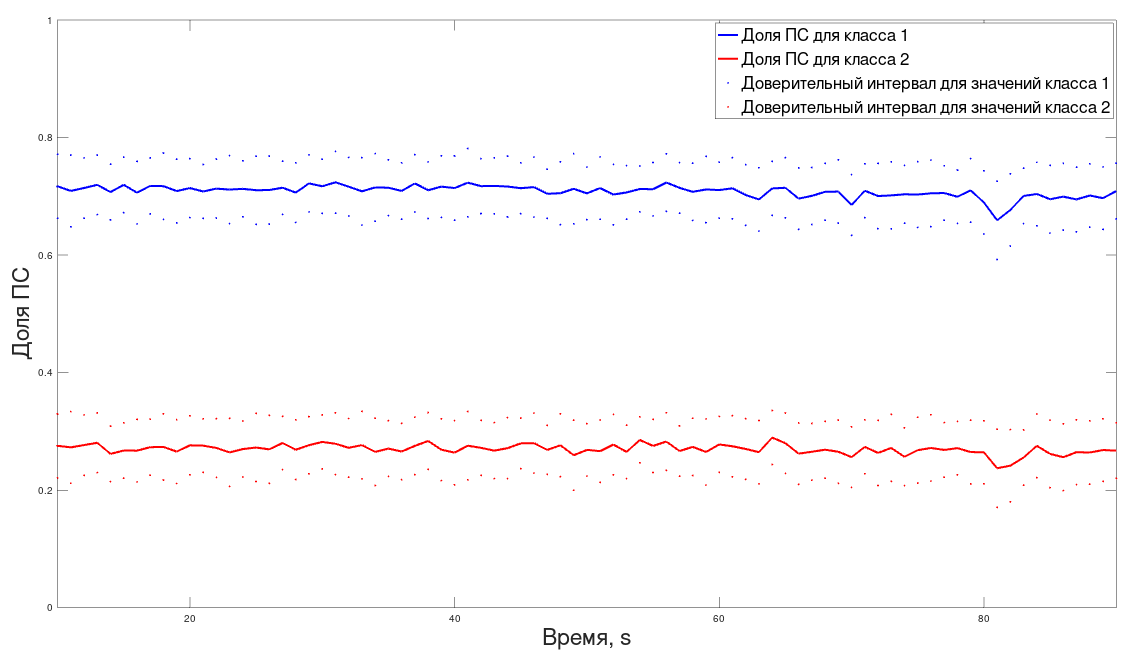
\includegraphics[scale=0.255]{./plotc.png}

	\end{figure}
	\begin{center}{\footnotesize
	 Среднее значение процента ПС для класса 1: $71 \pm 3 \%$ $(P = 0.95)$.\\
     Среднее значение процента ПС для класса 2: $27 \pm 2 \%$ $(P = 0.95)$.\\
	}
	\end{center}
\end{frame}

\begin{frame}[fragile]{Структура эксперимента №2}

{\footnotesize%
	\begin{lstlisting}[frame=single,emph={iperf3},emphstyle={\bfseries}]
iperf3 -c $SERVERIP -p $TESRPORT1 -b 100M -u -t 90
iperf3 -c $SERVERIP -p $TESRPORT2 -b 5M -u -t 90
    \end{lstlisting}%
}%

	\begin{figure}
		\center
    	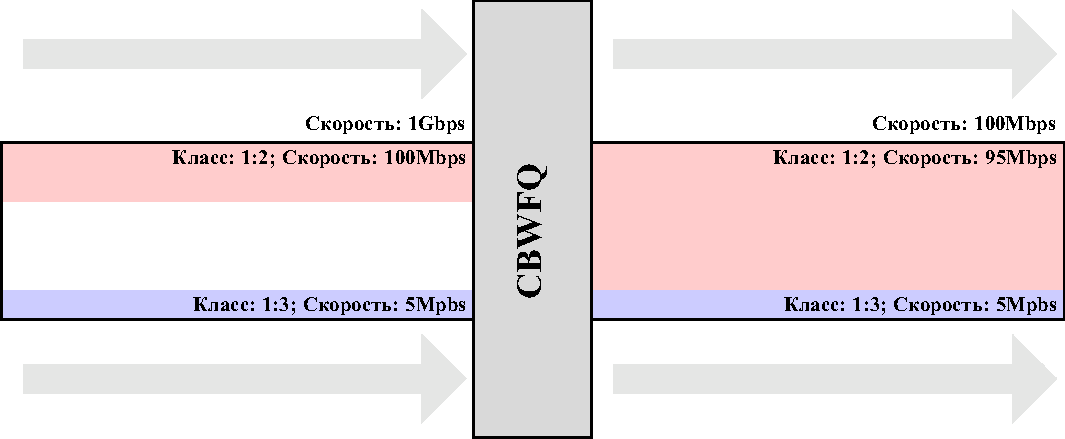
\includegraphics[scale=0.65]{../text/pdfimages/exp_scheme2.pdf}
	\end{figure}
\end{frame}

\begin{frame}{График распределения доли ПС по классам}
	\begin{figure}
		\center
    	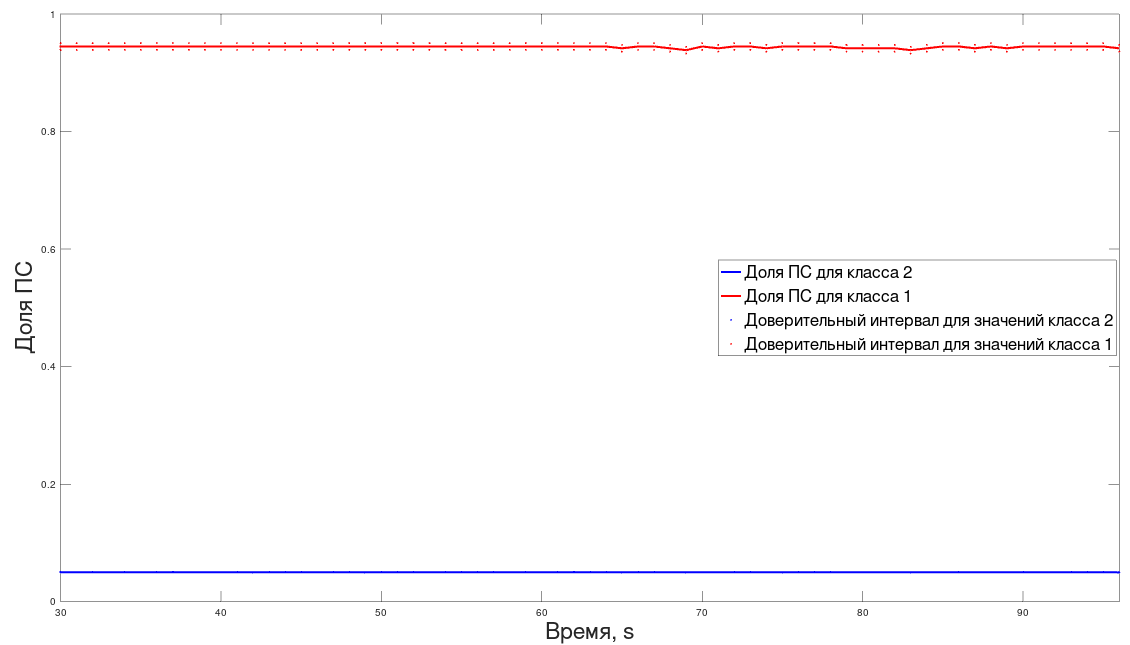
\includegraphics[scale=0.255]{./plotnc.png}

	\end{figure}
	\begin{center}
		{\footnotesize 
		 Среднее значение процента  ПС для класса 1: $94 \pm 0.5 \%$ $(P = 0.95)$.\\
         Среднее значение процента  ПС для класса 2: $5 \pm 0.07 \%$ $(P = 0.95)$.
		}
	\end{center}
\end{frame}


%\begin{frame}{Тестирование модуля}

%\end{frame}

\begin{frame}{Вывод}
	\begin{itemize}
		\item Проведён сравнительный анализ классовых дисциплин обслуживания.
		\item Проведено исследование модели WFQ.
		\item Реализован интерфейс для системы tc.
		\item Реализован алгоритм CBWFQ в ядре Linux.
		\item Перспектива развития работы: реализация алгоритма WRED и доработка модуля до дисциплины LLQ.
	\end{itemize}
\end{frame}

\itmothankyou

\end{document}
